\documentclass[12pt,a4paper,oneside]{article}
\usepackage[utf8]{inputenc}
\usepackage[english]{babel}
\usepackage{amsmath}
\usepackage{amsfonts}
\usepackage{amssymb}
\usepackage{graphicx}
\usepackage[]{algorithm2e}
\usepackage[left=2cm,right=2cm,top=2cm,bottom=2cm]{geometry}
%\usepackage{algorithm}
%\usepackage{algorithmic}

\begin{document}

\begin{center}
\textbf{\large{Report September 24th}} \\
\textbf{Improving the formalization of the algorithm and Building our architecture}
\end{center}

The basic input for the Rhone algorithm is: (1) a query; and (2) a list of concrete services.
Query and concrete service are formally defined as follows.

\noindent \textbf{Definition 1 (Query):} A query $Q$ has the form:
\begin{center}
$Q (\overline{I}, \overline{O}) := A_{1}(\overline{I}, \overline{O}), A_{2}(\overline{I}, \overline{O}), ..,  A_{n}(\overline{I}, \overline{O}),C_{1},C_{2}, .., C_{m}[P_{1},P_{2}, .., P_{k}]$
\end{center}  
The left side of the definition is the head of the query; and the right side is the body. 
$\overline{I}$ and $\overline{O}$ are a set of \textit{input} and \textit{output} parameters, respectively.
A query is expressed as set of abstract services ($A$) which specify abstract functions performed by the query.
%An abstract service is abstract function performed by the query. 
Constraints over the \textit{input} or \textit{output} parameters are defined in $C$.
The user preferences over the services are signed in $P$. $C$ and $P$ are in the form $x \otimes constant$ such that $\otimes \in\lbrace \geq, \leq, =, \neq, <, >\rbrace$.

\noindent \textbf{Definition 2 (Concrete service):} A concrete service ($S$) has its form similar to a query:
\begin{center}
$S (\overline{I}, \overline{O}) := A_{1}(\overline{I}, \overline{O}), A_{2}(\overline{I}, \overline{O}), ..,  A_{n}(\overline{I}, \overline{O})[P_{1},P_{2}, .., P_{k}]$
\end{center}  
A concrete service ($S$) is defined as a set of abstract services ($A$), and by its quality constraints $P$. 
These quality constraints associated to the service represent the service level agreement exported by the concrete service.

Given the query and the concrete services, the algorithm tries to match abstract services in $S$ with the same abstract service in $Q$. 

\noindent \textbf{Definition 3 (Abstract service equivalence):} Given an abstract service $A_{i}$ such that $A_{i} \in Q$ and $A_{i} \in S$. $A_{i}.Q$ is equivalent to $A_{i}.S$, denoted $A_{i}.Q = A_{i}.S$, iff (1) $A_{i}.Q$ and $A_{i}.S$ have the same abstract function name; (2) the number of \textit{input} and \textit{output} variables of $A_{i}.Q$ is equal to the same of $A_{i}.S$.

%\noindent \textbf{Definition 3 (Abstract service equivalence):} Given a query $Q$; a concrete service $S$; and an abstract service $A_{i}$ such that $A_{i} \in Q$ and $A_{i} \in S$, $A_{i}.Q$ is equivalent to $A_{i}.S$, denoted $A_{i}.Q = A_{i}.S$, iff the number of variables of $A_{i} \in Q$ is equal to the number of variables of $A_{i}.S$.

Once a matching between abstract services is found, the algorithm checks if the concrete service associated in the matching is a candidate to be part of the rewriting process.

\noindent \textbf{Definition 4 (Candidate service):} Given a query $Q$ and a concrete service $S$, $S$ is a candidate service iff: (1) $\nexists A_{i} \ s.t. \ A_{i} \in S \ and \ A_{i} \not\in Q$; and (2) the quality constraints in $S$ does not violate the user preferences in $Q$. 

%\noindent \textbf{Definition 4 (Candidate service):} Given a query $Q$ and a concrete service $S$, $S$ is a candidate service iff $\nexists A_{i} \ s.t. \ A_{i} \in S \ and \ A_{i} \not\in Q$. $\forall A_{i} \in S$ and an abstract service $A_{i}$ such that $A_{i} \in Q$ and $A_{i} \in S$, the mapping $A_{i}.Q \longmapsto A_{i}.S$ can be generated iff:
%(1) $A_{i}.Q = A_{i}.S$; and (2) $\nexists A \ s.t. \ A \in S \ and \ A \not\in Q$.

In the next step, the algorithm builds the \textit{partial descriptors} (PD). 
Each descriptor describes how a \textit{candidate} concrete service can be used in the query rewriting process.

\noindent \textbf{Definition 5 (Partial Descriptor):} PD is a complex data structure defined as follows: 
%\begin{center}
$\langle S, h, \varphi, G, P\rangle$
%\end{center}
where $S$ is a concrete service. 
\textit{h} are mappings between terms in the head of $S$ to terms in the body of $S$. 
$\varphi$ are mapping between terms from the abstract composition to terms in the concrete service definition.
$G$ is a set of abstract services covered by $S$. 
$P$ is a set quality constraints associated to the service $S$. 

Intuitively, a rewriting is a set of \textit{partial descriptors} that fully covers the original query, and do not violates the user preferences.

\begin{flushleft}
\textbf{Architecture}
\end{flushleft}

\textit{Query Generator Module} helps the user to create his queries, and to define his preferences. 
Once we have a query this module will try to find if there are previous rewritings to a equivalent query. 
If true, \textit{the composition and execution module} can publish and execute the new composition retrieving and integrating the new data.
If there are no previous rewritings, the module interacts with the \textit{service locator} in order to identify in our \textit{service registry} services that can answer the query or part of it.
The query and the selected services are used in the \textit{Query Rewriting Module} to generate the rewritings for the query. 
The rewritings are sent to \textit{the composition and execution module} to be published and executed (perhaps we can use BPEL to compose and execute).
The integration process could be done in our database or in the database of one related services (somehow we should analyze which one is the best option).

\begin{figure}[h]
\center
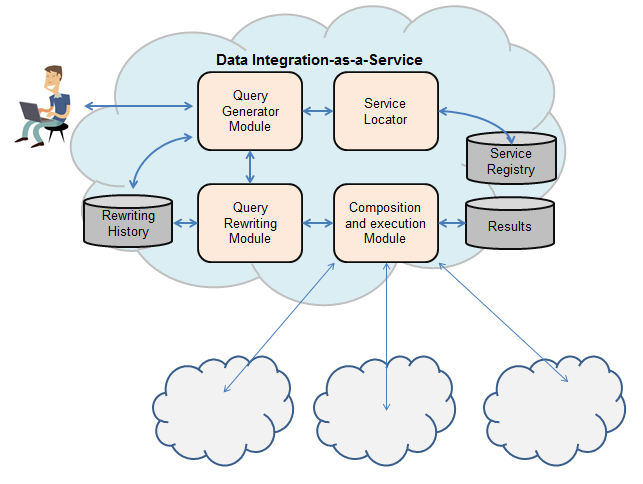
\includegraphics[scale=0.8]{arch.PNG} 
\end{figure}


%-------------
% 
%A concrete service ($S$) is defined as a set of abstract services ($A$), and by its quality constraints $P$. 
%These quality constraints associated to the service represent the service level agreement exported by the concrete service.
%
%
%The \textbf{input data} for the algorithm is a query (Q) and a list of concrete services (C1, C2, ...). The query and concrete services are defined as follows:
%
%
%\begin{figure}[h]
%\center
%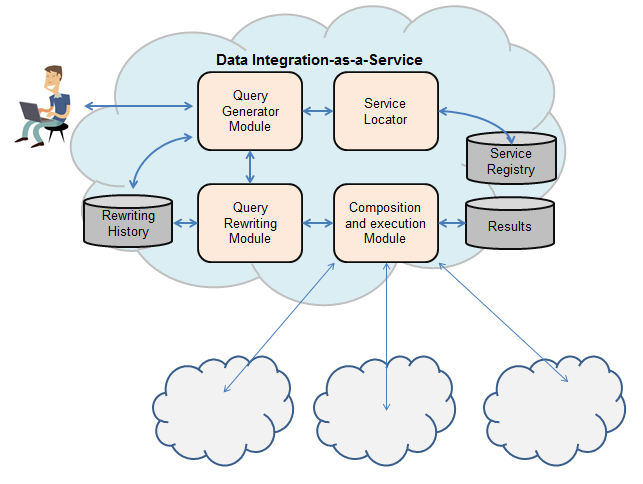
\includegraphics[scale=0.8]{arch.PNG} 
%\end{figure}
%
%
%
%The query and concrete services are defined as a set of abstract services ($A_{1}, A_{2}, ..., A_{n}$) and a set of quality constraints ($Q_{1},Q_{2}, ..., Q_{n}$). $\overline{t}$ is a set of input (decoration \textbf{?}) or output (decoration \textbf{!}) variables. The first \textbf{processing step} of the algorithm creates the data structures that represent the query and concrete services. The query and concrete service data structure will be formed by its $name$, a set of head variables ($V_{h}$) and a set of abstract services ($A_{s}$).
%
%\begin{center}
%$Q = \langle name, V_{h}, A_{s} \rangle$ \\
%$C = \langle name, V_{h}, A_{s} \rangle$
%\end{center}
%
%For each abstract service A in the set $A_{s}$, a data structure containing its $name$ and a set of variables ($V$) is build. Notice that the set of variables ($V$) can contain head variables or local variables.
%
%\begin{center}
%$A = \langle name, V\rangle$
%\end{center}
%
%Once these structures were created, the \textbf{second step in the algorithm is to form the PCDs}. PCDs are created only for those concrete services which have abstract services that can answer that query or part of it. PCDs are defined as follows:
%
%\begin{center}
%$\langle S, h, \varphi, G, Def, has\_opt\rangle$
%\end{center}
%
%\textbf{\textit{S}} is a concrete service. \textit{h} are mapping between terms in the head of the service definition to terms in the right side of the service definition. \textbf{\textit{$\varphi$}} are mapping between terms from the abstract composition to terms in the concrete service definition. \textbf{\textit{G}} is a set of abstract services names and quality constraints covered by \textbf{\textit{S}}. \textbf{\textit{Def}} is a set conditions that are not covered by \textbf{\textit{S}} alone.\textbf{ \textit{has\_opt}} is a boolean flag to indicate that some abstract service in the definition of \textbf{\textit{S}} has been used in \textbf{\textit{G}} and has an optional parameter.
%
%After that, all the \textbf{PCDs formed in the previous step are combined}. Once we have all the possible combinations of PCDs, \textbf{each combination is verified} to confirm if the combination is a valid rewriting of the former query or not.
%A valid rewriting is a list of PCDs that answers the complete query without redundancies, and without more than one mapping to the same variable with distinct values.
%\bigskip
%Considering that we have the data structure for the query (Q) and concrete services (C), the general idea of the algorithm is defined in the function \emph{rewriting}:
%
%\begin{verbatim}
%function rewriting (Q, C)
%   l := createPCDs(Q, C)
%   P := combinePCD (l)
%foreach p in P
%   if isRewriting(Q,p)
%      R := R U {p}
%return R
%\end{verbatim}
%
%\begin{algorithm}[H]
% \KwData{this text}
% \KwResult{how to write algorithm with \LaTeX2e }
% initialization\;
% \While{not at end of this document}{
%  read current\;
%  \eIf{understand}{
%   go to next section\;
%   current section becomes this one\;
%   }{
%   go back to the beginning of current section\;
%  }
% }
% \caption{How to write algorithms}
%\end{algorithm}
%
%
%The function \emph{createPCDs} returns a list of PCDs \textbf{l}. \textbf{P} is a list all possible combinations of PCDs returned by the function \emph{combinePCD}. And, for each PCD combination in \textbf{P}, the function \emph{isRewriting} verifies the combination is a valid rewriting or not. If true, the set of rewriting \textbf{R} is updated adding the new combination. In the end, the list of rewriting \textbf{R} is returned.
%
%\bigskip The examples next show the data structure created for input data, the intermediary data generated while processing the algorithm, and the output rewriting expected.
% 
%\begin{flushleft}
%\textbf{Describing an example 1}
%\end{flushleft}
%
%\begin{flushleft}
%\textbf{Query:} \\
%Q(disease?, patients!, dnas!, birth!, gen!, addr!, wheatherstatistic!) :- A1(disease?, patients!), A2(patients?,dnas!), A3(patients?, birth!, gen!, addr!), A4(addr?, wheatherstatistic!) \\
%\end{flushleft}
%
%The data created for the query above is:
%
%\begin{center}
%$\langle Q, [disease?, patients!, dnas!, birth!, gen!, addr!, wheatherstatistic!], [A1,A2,A3,A4] \rangle$
%\end{center}
%
%For each abstract service the following data is created:
%
%\begin{flushleft}
%$\langle A1, [disease?, patients!]\rangle$ \\
%$\langle A2, [patients?,dnas!]\rangle$ \\
%$\langle A3, [patients?, birth!, gen!, addr!]\rangle$ \\
%$\langle A4, [addr?, wheatherstatistic!]\rangle$ \\
%\end{flushleft}
%
%The same procedure is done for the concrete services.
%
%\begin{flushleft}
%\textbf{Concrete services:} \\
%S1(d?, p!) :- A1(d?, p!)\\
%S2(d?, p!) :- A1(d?, p!)\\
%S3(p?, d!) :- A2(p?, d!)\\
%S4(p?, dateofbirth!, gender!, address!) :- A3(p?, dateofbirth!, gender!, address!)\\
%S5(address?, wheatherstaticalinformation!) :- A4(address?, wheatherstaticalinformation!)\\
%S6(p?, d!) :- A5(p?, d!)\\
%S7(p?, vaccinateddiseases!) :- A6(p?, vaccinateddiseases!)\\
%\end{flushleft}
%
%Once we have all the data structure created, PCDs for abstract services that can solve the query will be created. Such as:
%
%\begin{flushleft}
%$\langle S1, [d? \longmapsto d?, p! \longmapsto p!], [d? \longmapsto disease?, p! \longmapsto patients!], A1, \emptyset, false\rangle$ \\
%$\langle S2, [d? \longmapsto d?, p! \longmapsto p!], [d? \longmapsto disease?, p! \longmapsto patients!], A1, \emptyset, false\rangle$ \\
%$\langle S3, [p? \longmapsto p?, d! \longmapsto d!], [p? \longmapsto patients?, d! \longmapsto dnas!], A2, \emptyset, false\rangle$ \\
%$\langle S4, [p? \longmapsto p?, dateofbirth! \longmapsto dateofbirth!, gender! \longmapsto gender!, address! \longmapsto address!], [p? \longmapsto patients?, dateofbirth! \longmapsto birth!, gender! \longmapsto gen!, address! \longmapsto addr!], A3, \emptyset, false\rangle$ \\
%$\langle S5, [address? \longmapsto address?, wheatherstaticalinformation! \longmapsto wheatherstaticalinformation!], [address? \longmapsto addr?, wheatherstaticalinformation! \longmapsto wheatherstatistic!], A4, \emptyset, false\rangle$ \\
%\end{flushleft}
%
%Based on these PCDs, all possible combination are created, and then the valid ones are returned as rewriting of the former query. The expected \textbf{rewriting results} are:
%
%\begin{flushleft}
%\textbf{1) }Q(disease,patients,dnas,birth,gen,addr,wheatherstatistic) :- S1(disease,patients),S3(patients,dnas),S4(patients,birth,gen,addr),S5(addr,wheatherstatistic) \\
%\textbf{2) }Q(disease,patients,dnas,birth,gen,addr,wheatherstatistic) :- S2(disease,patients),S3(patients,dnas),S4(patients,birth,gen,addr),S5(addr,wheatherstatistic) \\
%\end{flushleft}
%
%\begin{flushleft}
%\textbf{Describing an example 2}
%\end{flushleft}
%
%The difference between the example 1 and 2 is the concrete service S2. Now, I defined it being able to solve two parts in the query.
%
%\begin{flushleft}
%\textbf{Query:} \\
%Q(disease?, patients!, dnas!, birth!, gen!, addr!, wheatherstatistic!) :- A1(disease?, patients!), A2(patients?,dnas!), A3(patients?, birth!, gen!, addr!), A4(addr?, wheatherstatistic!) \\
%\end{flushleft}
%
%\begin{flushleft}
%\textbf{Concrete services:} \\
%S1(d?, p!) :- A1(d?, p!)\\
%S2(d?, p!, dna!) :- A1(d?, p!), A2(p?, dna!)\\
%S3(p?, d!) :- A2(p?, d!)\\
%S4(p?, dateofbirth!, gender!, address!) :- A3(p?, dateofbirth!, gender!, address!)\\
%S5(address?, wheatherstaticalinformation!) :- A4(address?, wheatherstaticalinformation!)\\
%S6(p?, d!) :- A5(p?, d!)\\
%S7(p?, vaccinateddiseases!) :- A6(p?, vaccinateddiseases!)\\
%\end{flushleft}
%
%Note the difference in the PCD for S2 in the following lines. Now the set \textbf{G} has indications for A1 and A2.
%
%\begin{flushleft}
%$\langle S1, [d? \longmapsto d?, p! \longmapsto p!], [d? \longmapsto disease?, p! \longmapsto patients!], A1, \emptyset, false\rangle$ \\
%$\langle S2, [d? \longmapsto d?, p! \longmapsto p!, dna! \longmapsto dna!], [d? \longmapsto disease?, p! \longmapsto patients!, dna! \longmapsto dnas!], \lbrace A1,A2 \rbrace, \emptyset, false\rangle$ \\
%$\langle S3, [p? \longmapsto p?, d! \longmapsto d!], [p? \longmapsto patients?, d! \longmapsto diseases!], A2, \emptyset, false\rangle$ \\
%$\langle S4, [p? \longmapsto p?, dateofbirth! \longmapsto dateofbirth!, gender! \longmapsto gender!, address! \longmapsto address!], [p? \longmapsto patients?, dateofbirth! \longmapsto birth!, gender! \longmapsto gen!, address! \longmapsto addr!], A3, \emptyset, false\rangle$ \\
%$\langle S5, [address? \longmapsto address?, wheatherstaticalinformation! \longmapsto wheatherstaticalinformation!], [address? \longmapsto addr?, wheatherstaticalinformation! \longmapsto wheatherstatistic!], A4, \emptyset, false\rangle$ \\
%\end{flushleft}
%
%Based on these PCDs, the expected \textbf{rewriting results} are:
%
%\begin{flushleft}
%\textbf{1) }Q(disease,patients,dnas,birth,gen,addr,wheatherstatistic) :- S1(disease,patients),S3(patients,dnas),S4(patients,birth,gen,addr),S5(addr,wheatherstatistic) \\
%\textbf{2) }Q(disease,patients,dnas,birth,gen,addr,wheatherstatistic) :- S2(disease,patients,dnas),S4(patients,birth,gen,addr),S5(addr,wheatherstatistic) \\
%\end{flushleft}


\end{document}